\documentclass{article}
\usepackage[utf8]{inputenc}
\usepackage[english, swedish]{babel}

\usepackage{cite}
\usepackage{caption}
\usepackage{graphicx}
\usepackage{float}
\usepackage{textcomp}
\usepackage[yyyymmdd]{datetime}
\renewcommand{\dateseparator}{-}

\usepackage{graphicx}
\graphicspath{ {images/} }

%For headers & footers
\usepackage{fancyhdr}
\pagestyle{fancy}
\lhead{
\includegraphics[scale=0.2]{Logo}}
\chead{Kartrobot}
\rhead{\today}

\lfoot{Konstruktion med mikrodatorer}
\rfoot{Grupp 3}

\renewcommand{\headrulewidth}{0.4pt}
\renewcommand{\footrulewidth}{0.4pt}


\title{Teknisk dokumentation för kartrobot}
\author{Patrik Sletmo}
\date{\today}

\selectlanguage{swedish}

\begin{document}

\thispagestyle{empty}

{
\sffamily
\centering
\large


{\huge 
Teknisk dokumentation för kartrobot
}

{\large
Patrik Sletmo
}

{\large
Version 1.0
}

\vspace{3.5cm}

Status
\begin{table}[H]
\centering
\begin{tabular}{ | c | c | c | }
\hline
STATUS & Patrik Sletmo & 2016-12-DD \\
\hline
\end{tabular}
\end{table}
}
\clearpage

\vspace*{\fill}
{
\sffamily
\centering
\large


{\huge
Projektidentitet
}

{\large
Grupp 3, 16/HT, KarToffel \\ Linköpings tekniska högskola, ISY
}

\vspace{0.5cm}

\begin{table}[H]
\centering
\begin{tabular}{ | c | c | c | c |}
\hline
Namn & Ansvar & Telefon & E-post \\
\hline
Patrik Sletmo & Projektledare & 070 783 57 61 & patsl736@student.liu.se \\
\hline
Rebecca Lindblom & Utvecklare & 073 436 40 79 & rebli156@student.liu.se \\
\hline
Matildha Sjöstedt & Utvecklare & 070 515 84 11 & matsj696@student.liu.se \\
\hline
Sebastian Callh & Utvecklare & 073 820 46 64 & sebca553@student.liu.se \\
\hline
Anton Dalgren & Utvecklare & 076 836 51 56 & antda685@student.liu.se \\
\hline
Matilda Dahlström & Utvecklare & 070 636 33 52 & matda715@student.liu.se \\
\hline
\end{tabular}
\end{table}
}

\begin{center}
\textbf{Hemsida}: https://github.com/SebastianCallh/kartoffel-tsea29
\end{center}

\begin{center}
\textbf{Kund}: Mattias Krysander, 013 - 28 2198 , matkr@isy.liu.se
\end{center}

\begin{center}
\textbf{Kursansvarig}: Tomas Svensson, 3B 528, +46 (0)13 28 1368, tomas.svensson@liu.se \\
\textbf{Handledare}: Anders Nilsson, 3B 512, +46 (0)13 28 2635, anders.p.nilsson@liu.se
\end{center}
\vspace*{\fill}
\clearpage

\renewcommand*\contentsname{Innehållsförteckning}
\tableofcontents
\clearpage


{
\sffamily
\centering
\large


{\huge 
Dokumenthistorik \\
}
\begin{table}[H]
\centering
\begin{tabular}{ | c | c | c | c | c |} 
\hline
\textbf{Version} & \textbf{Datum} & \textbf{Utförda ändringar} & \textbf{Utförd av } & \textbf{Granskad} \\
\hline
VERSION & 2016-12-DD & Första version & Grupp 3 & Patrik Sletmo \\
\hline

\end{tabular}
\end{table}
}

\clearpage

\section{Inledning}
% Kort beskrivning av hela dokumentet, skrivs förslagsvis sist

\section{Systembeskrivning}
% Beskrivning av systemets mest framträdande egenskaper
Systemet består av en fyrhjulig robot samt en mjukvaruklient som kommunicerar med varandra via bluetooth.
Syftet med systemet är att roboten ska kunna kunna kartlägga sin omgivning helt autonomnt. För att göra det 
så har den diverse IR-sensorer, en lasersensor och ett gyroskop monterat på sig för att kunna navigera och mäta avstånd.
Bluetooth-kopplingen låter mjukvaruklienten se kartläggningen i realtid, och ger möjligheten att fjärrstyra roboten.

\subsection{Delsystem}
% Upplistning av delsystem, eventuellt någon kort kommentar om varje delsystem
Hela systemet är moduluppbyggt, och består av följande delsystem:
\begin{itemize}
\item Mjuvaruenhet
\item Huvudenhet
\item Sensorenhet
\item Styrenhet
\end{itemize}

\subsection{Övergripande konstruktion}
% Övergripande blockschema
\begin{figure}[H]
\centering

\includegraphics[scale=0.4]{Logo}
\caption{Översikt över systemet}
\label{fig:oversikt_systemet3}
\end{figure}

TODO:TEXT OM ÖVERGRIPANDE KONSTRUKTION OCH FIGUR

\subsection{Komponenter}
% Väldigt kort beskrivning av delsektion
Här nedan listas alla komponenter som roboten består av.

\subsubsection{Beräkningsenheter}
% Upplistning av processorer, SOC:s, etc
\begin{table}[H]
  \centering
  \begin{tabular}{ | c | c | c | c |}
    \hline
    \textbf{Enhet} & \textbf{Antal} \\
    \hline
    Raspberry Pi 3 & 1 \\
    \hline
    ATMega 1284 & 2 \\
    \hline
  \end{tabular}
  \caption{ Tabell över beräkningsenheter. }
\end{table}

\subsubsection{Sensorer}
% Upplistning av alla sensorer
\begin{table}[H]
  \centering
  \begin{tabular}{ | c | c | c | c |}
    \hline
    \textbf{Komponent} & \textbf{Antal} \\
    \hline
    LIDAR-Lite v2 & 1 \\
    \hline
    Knapp & 1 \\
    \hline
    GP2Y0A41SK IR-Sensor & 3 \\
    \hline
    GP2Y0A21 IR-Sensor & 1 \\
    \hline
    Adafruit 10-DOF IMU & 1 \\
    \hline
  \end{tabular}
  \caption{ Tabell över sensorer. }
\end{table}

\subsubsection{Ställdon}
% Servon, motorer, etc
\begin{table}[H]
  \centering
  \begin{tabular}{ | c | c | c | c |}
    \hline
    \textbf{Komponent} & \textbf{Antal} \\
    \hline
    291RPM DC-motor & 4 \\
    \hline
  \end{tabular}
  \caption{ Tabell över ställdon. }
\end{table}


\subsubsection{IC-kretsar}
% Shifters
\begin{table}[H]
  \centering
  \begin{tabular}{ | c | c | c | c |}
    \hline
    \textbf{Komponent} & \textbf{Antal} \\
    \hline
    BSS138 & 1 \\
    \hline
  \end{tabular}
  \caption{ Tabell över IC-kretsar. }
\end{table}

\clearpage
\section{Delsystem}

\subsection{Huvudenhet}
Huvudenheten består till hårdvaran av en Raspberry PI, på vilken operativsystemet Raspbian körs. Den representerar robotens beslutsfattande organ och sköter navigationsbeslut, kartläggning, kommunikation med mjukvaruklienten samt agerar mästare på robotens I2C-buss. 

\subsubsection{Delsystemets funktion}
Huvudenheten är uppdelad i två undermoduler, logikenheten och kommunikationsenheten. Logikenheten analyserar data från sensorenheten för att avgöra hur roboten ska navigera och för att bestämma hur omvärlden ser ut så att den kan kartläggas. Roboten följer väggen på höger sida och genom att göra det kartlägger den hela den utomliggande väggen. När vi väl avgränsat rummet och området som köksön kan befinna sig i så vet roboten att de väggsegment den upptäckt som inte ingår i den utomliggande väggen är en del av köksön, och kan på så sätt navigera till dem och kartlägga därifrån. När hela kartan finns i robotens minne återvänder den till dess startposition. Logikenheten ansvarar även för att hålla koll på var någonstans i rutnätet roboten befinner sig. Kommunikationsenheten agerar som ett abstraktionslager för Raspberry Pi:ens Bluetoothmodul och ser till att sköta all översättning där i mellan så att systemet kan arbeta med interna dataformat i övriga delar.

\subsubsection{Kopplingsschema}
\begin{figure}[H]
\centering
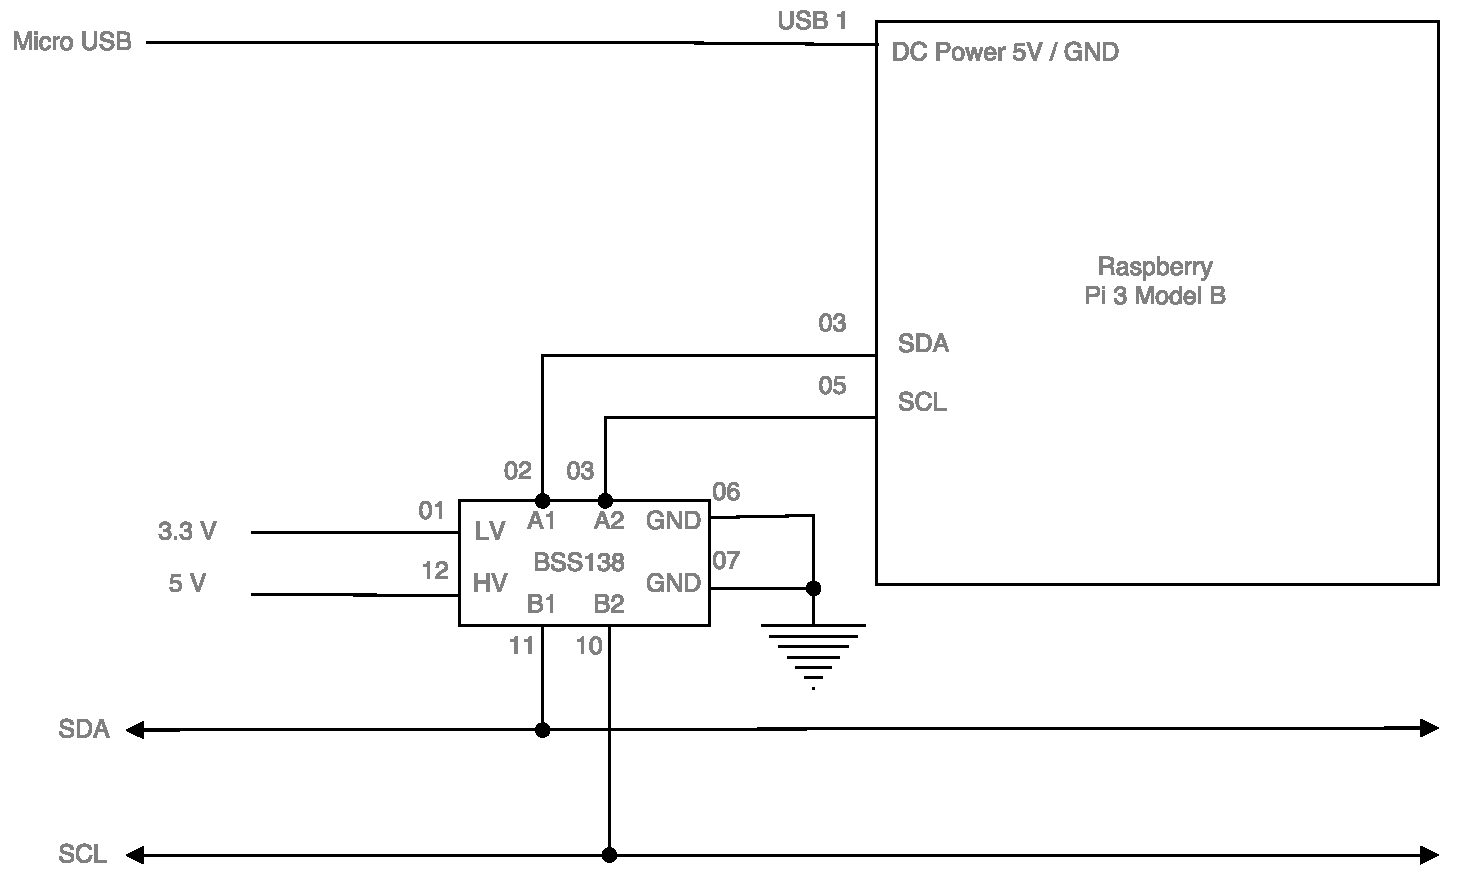
\includegraphics[scale=0.45]{Huvudenhet_kopplingsschema}
\caption{Kopplingsschema för huvudenheten.}
\label{fig:huvudenhet_kopplingsschema}
\end{figure}

Huvudenheten består av en Raspberry Pi 3 och en LCD-display av modellen JM162A. Utöver kopplingen till LCD:n så kopplas två pins till I2C-bussen.
Eftersom Raspberry Pi drivs av 3.3 V matspänning och de övriga atmega-processorerna i roboten drivs av 5 V så behövs vi nivåskifta bussen så att de kan kommunicera med varandra, vilket görs med nivåskiftaren BSS138.


\subsubsection{Komponenter}

\begin{table}[H]
   \centering
  \begin{tabular}{ | c | c | }
    \hline
    \textbf{Komponent} & \textbf{Antal} \\
    \hline
    Raspberry PI 3 & 1 \\
    \hline
    JM162A & 1 \\
    \hline
  \end{tabular}
\end{table}

\subsubsection{Resurser}


\begin{table}[H]
   \centering
  \begin{tabular}{ | c | c | c | }
    \hline
    \textbf{Port} & \textbf{Antal} & \textbf{Används} \\
    \hline
    GPIO pins & 40 & 12 \\
    \hline
  \end{tabular}
\end{table}


\subsubsection{Programflöde}
Programflödet i huvudenheten består i huvudsak av två delar: Den logiska delen som sköter navigeringsbesluten utifrån beräknad kartdata, samt delen som sköter kommunikation med resten av systemets delmoduler. Nedan beskrivs flödesscheman för navigering samt Bluetooth-kommunikation med huvudenheten. För detaljer kring kommunikation mellan huvud-, styr- och sensorenhet se avsnitt~\ref{sec:kommunikation_mellan_delsystem}. 
\begin{figure}[H]
\centering
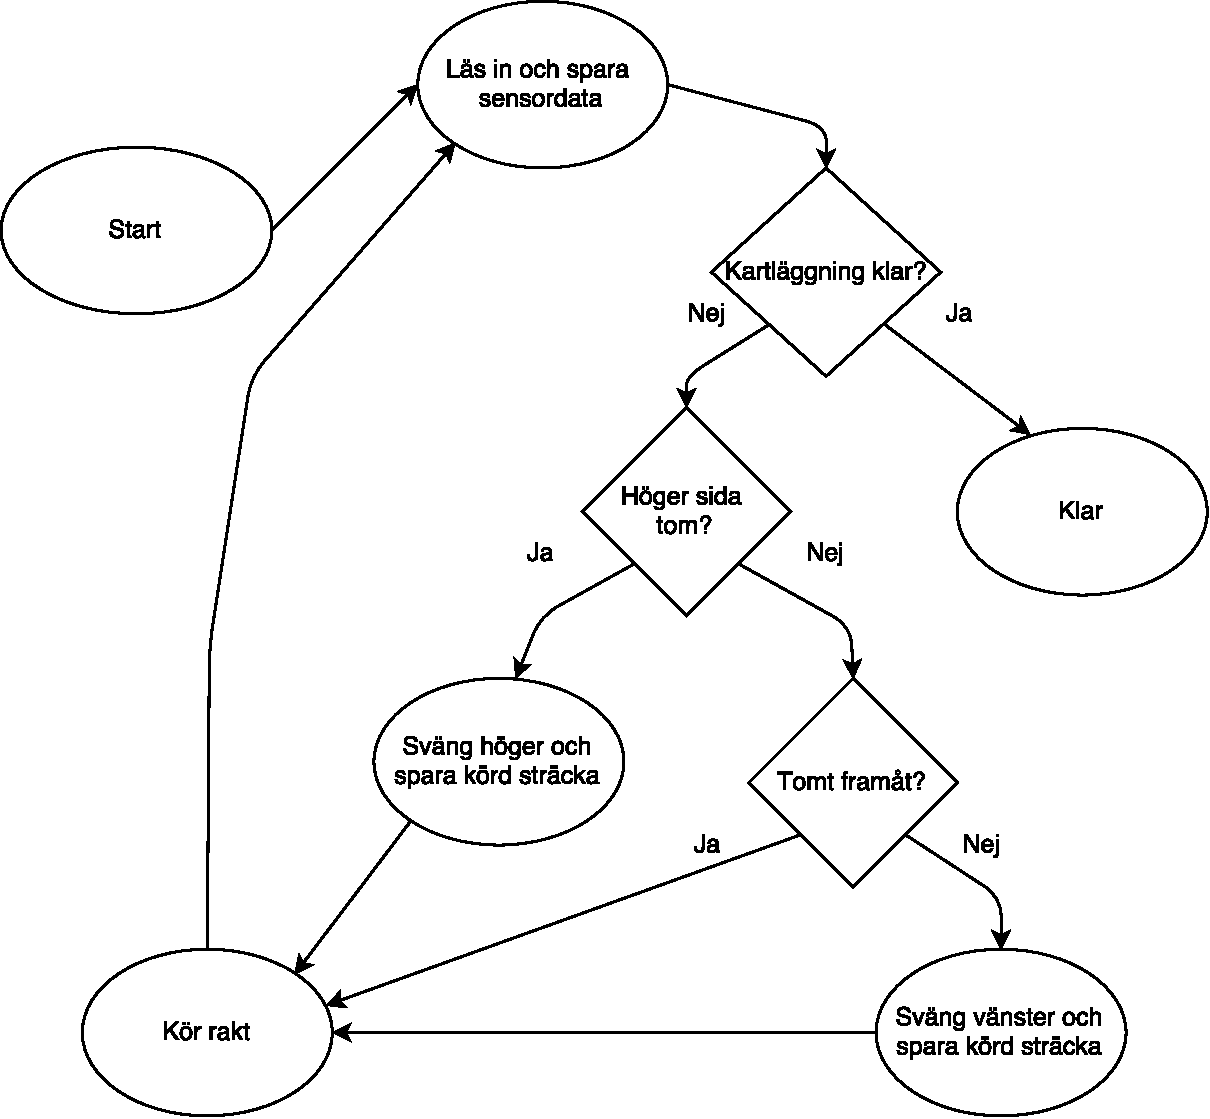
\includegraphics[scale=0.6]{navigering_flowchart}
\caption{Flödesdiagram för navigering.}
\label{fig:navigering_flowchart}
\end{figure}
\ \\

Roboten navigerar enligt flödesschemat i figur~\ref{fig:navigering_flowchart} till kartläggningen av rummets väggar är klara, det vill säga till det att den har cirkulerat hela rummet. Roboten vet med säkerhet att den under den här perioden kommer upptäcka väggsegment som ingår i köksön och inte i rummets väggar på sin västersida, och navigerar då till dem och påbörjar samma procedur som i flödesschemat igen varpå kartläggningen är klar.

\begin{figure}[H]
\centering

\includegraphics[scale=0.45]{Logo}
\caption{Flödesschema över Bluetooth-kommunikationen i huvudenheten.}
\label{fig:Kommunikation_huvudenhet_v2}
\end{figure}
\ \\

TODO:TEXT OM BLUETOOTH. UPPDATERA SÅ DEN REFLEKTERAR VÅR IMPLEMENTATION

\subsection{Sensorenhet}
% Se kommentarer för huvudenhet
Sensorenheten har i uppgift att läsa in värden från sensorerna som finns placerade på roboten och rapportera värdena till huvudenheten. Den består av fyra IR-sensorer, ett gyroskop och en lasersensor.

\subsubsection{Delsystemets funktion}
Sensorenhetens har sin egna beräkningsenhet, ATMega 1284, vilket låter den arbeta asynkront från våra andra enheter. Den ser på så sätt alltid till att ha data tillgänglig närhelst huvudenheten begär den. För IR-sensorerna sker det genom att processorn pollar information från varje sensor och sparar undan i minnet, medan gyroskop och laser håller koll på sina egna värden och är kopplade direkt på I2C-bussen. Huvudenheten kan sedan fråga sensorenheten efter ny IR-mätdata, eller fråga gyroskopet/lasern direkt varpå den får sensordatan levererad över I2C.

Avläsningarna från IR-sensorerna är analoga, och konverteras till digitalt med hjälp av ATMegans interna AD-omvandlare. För att sedan omvandla mätdatan till en approximation i millimeter används en tabell sparad i ATMegans minne.


\subsubsection{Kopplingsschema}
\begin{figure}[H]
\centering
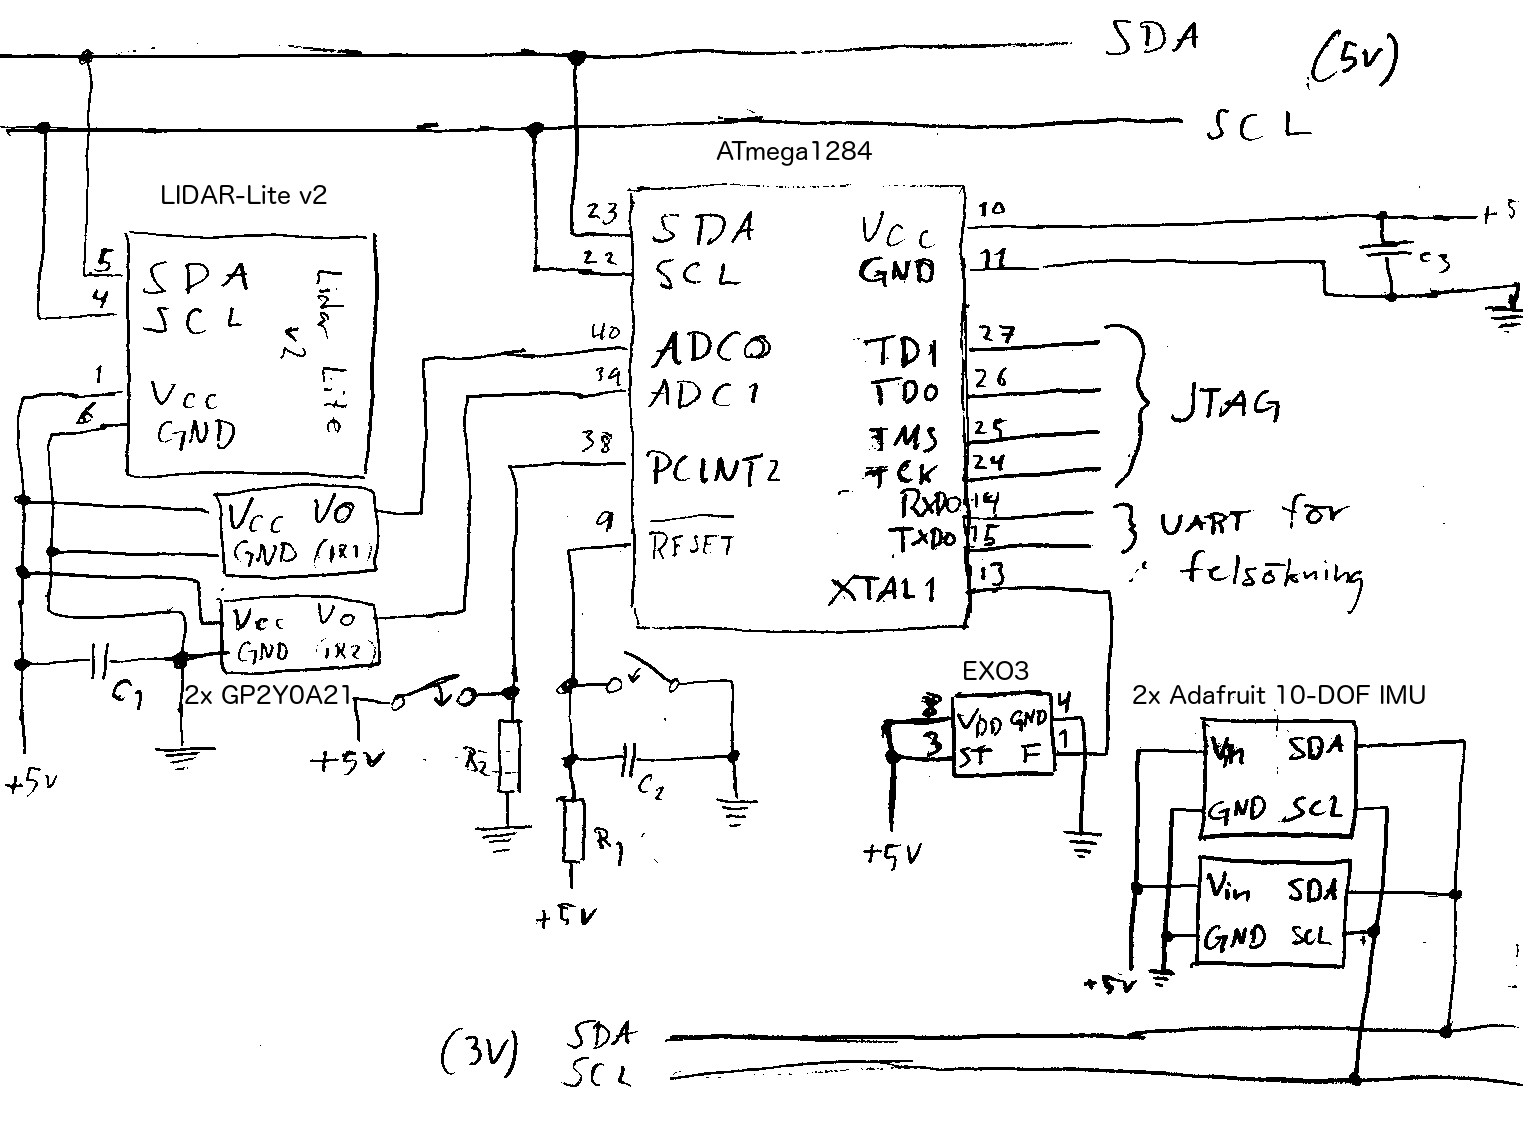
\includegraphics[scale=0.6]{Sensorenhet_kopplingsschema}
\caption{Kopplingsschema för sensorenheten.}
\label{fig:sensorenhet_kopplingsschema}
\end{figure}

Som ses i figur~\ref{fig:sensorenhet_kopplingsschema} är IR-sensorerna kopplade till ATMegan via var sitt lågpassfilter för att reducera brus. Längst upp i kopplingsschemat ses den gemensamma I2C-bussen, dit gyroskop och laser är anslutna. Notera att EXO3-komponenten är delad mellan sensorenheten och styrenheten trots att den illustreras som separata komponenter i kopplingsschemat.

\subsubsection{Komponenter}

\begin{table}[H]
  \centering
  \begin{tabular}{ | c | c | c | c |}
    \hline
    \textbf{Komponent} & \textbf{Antal} \\
    \hline
    ATMega 1284 & 1 \\
    \hline
    LIDAR-Lite v2 & 1 \\
    \hline
    Knapp & 1 \\
    \hline
    GP2Y0A41SK IR-Sensor & 3 \\
    \hline
    GP2Y0A21 IR-Sensor & 1 \\
    \hline
    Adafruit 10-DOF IMU & 1 \\
    \hline
    EXO3 & 1 (delad) \\
    \hline
  \end{tabular}
  \caption{ Tabell över de komponenter som sensorenheten består av. }
\end{table}

\subsubsection{Resurser}
% Rada upp tillgängliga portar på mikroprocessorn samt hur många som krävs
% Motivera val av mikroprocessor med uppskattning av de resurser som krävs (prestanda, minne, IO)

TODO:TABELLEN NEDAN EJ KORRIGERAD
\begin{table}[H]
  \centering
  \begin{tabular}{ | c | c | c | c |}
    \hline
    \textbf{Port} & \textbf{Antal} & \textbf{Krävs} \\
    \hline
    SDA & 1 & 1 \\
    \hline
    SCL & 1 & 1 \\
    \hline
    PCINT & 24 & 1 \\
    \hline
    A/D & 8 & 2 \\
    \hline
    RESET & 1 & 1 \\
    \hline
    USART & 4 & 2 \\
    \hline
    JTAG & 1 & 1 \\
    \hline
    CLK & 1 & 1 \\
    \hline
  \end{tabular}
  \caption{Tabell över tillgängliga portar på processorn.}
\end{table}

Den maximala hastigheten som sensordata kan läsas in i är begränsad av sensorernas rapporteringsfrekvens som är betydligt långsammare än en ATmega 1284:s klockfrekvens, därför lönar det sig inte med en snabbare processor för sensorenhetens syfte. Det i princip enda minnet sensorenheten använder sig av är för temporärlagring av alla IR-sensorers data, vilket endast motsvarar fyra heltal. Utöver sensorinläsningen kommer enheten svara på kommandon över huvudbussen som inte heller kräver några höga hastigheter eller minneskrav.

\subsubsection{Programflöde}

\begin{figure}[H]
\centering
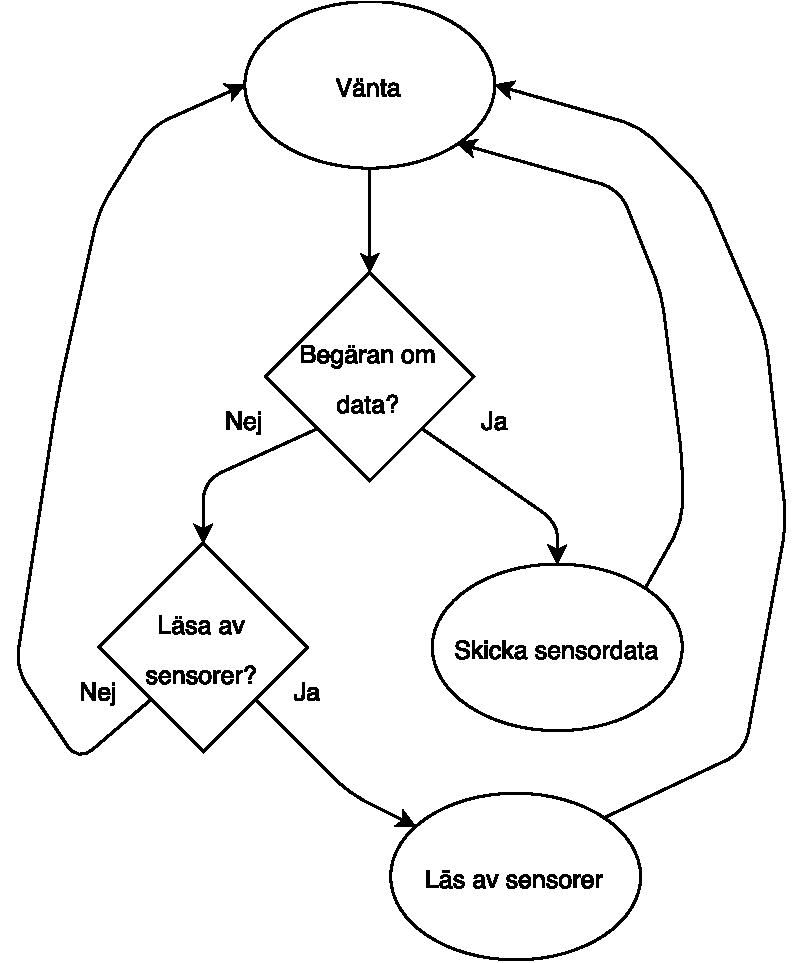
\includegraphics[scale=0.6]{sensorenhet_flowchart}
\caption{Ett flödesdiagram över sensorenhetens tillstånd}
\label{fig:sensorenhet_flowchart}
\end{figure}

För att kunna tillhandahålla sensordata från IR-sensorerna när huvudenheten ber den om det så läser sensorenheten in data med jämna mellanrum och sparar den lokalt för att sedan skicka datan på kommando från huvudenheten. Om den fått en begerän om sensordata från huvudenheten så tar det prioritet att leverera den över att läsa in ny data. Ett flödesdiagram över dess beteende ses i ~\ref{fig:sensorenhet_flowchart}.

\subsection{Styrenhet}
% Se kommentarer för huvudenhet
Styrenhetens uppgift är att kontrollera alla robotens fysiska rörelser med hjälp av servon, baserat på kommandon ifrån huvudenheten. Det är genom styrenhetens funktionalitet som roboten förflyttar sig igenom rummet som ska kartläggas.

\subsubsection{Delsystemets funktion}
Styrenheten består av en ATMega 1284 processor som har robotens alla servon kopplade till sig. Den tar emot kommandon från huvudenheten över I2C-bussen som säger åt roboten att exempelvis åka framåt eller rotera. Som svar skickar styrenheten ut korrekta signaler till relevanta servon för att kontrollera robotens rörelser enligt instruktioner.

För att styra robotens hjul används PWM, där styrenheten är förprogrammerad med lämplig pulskvot.

\subsubsection{Kopplingsschema}
\begin{figure}[H]
\centering
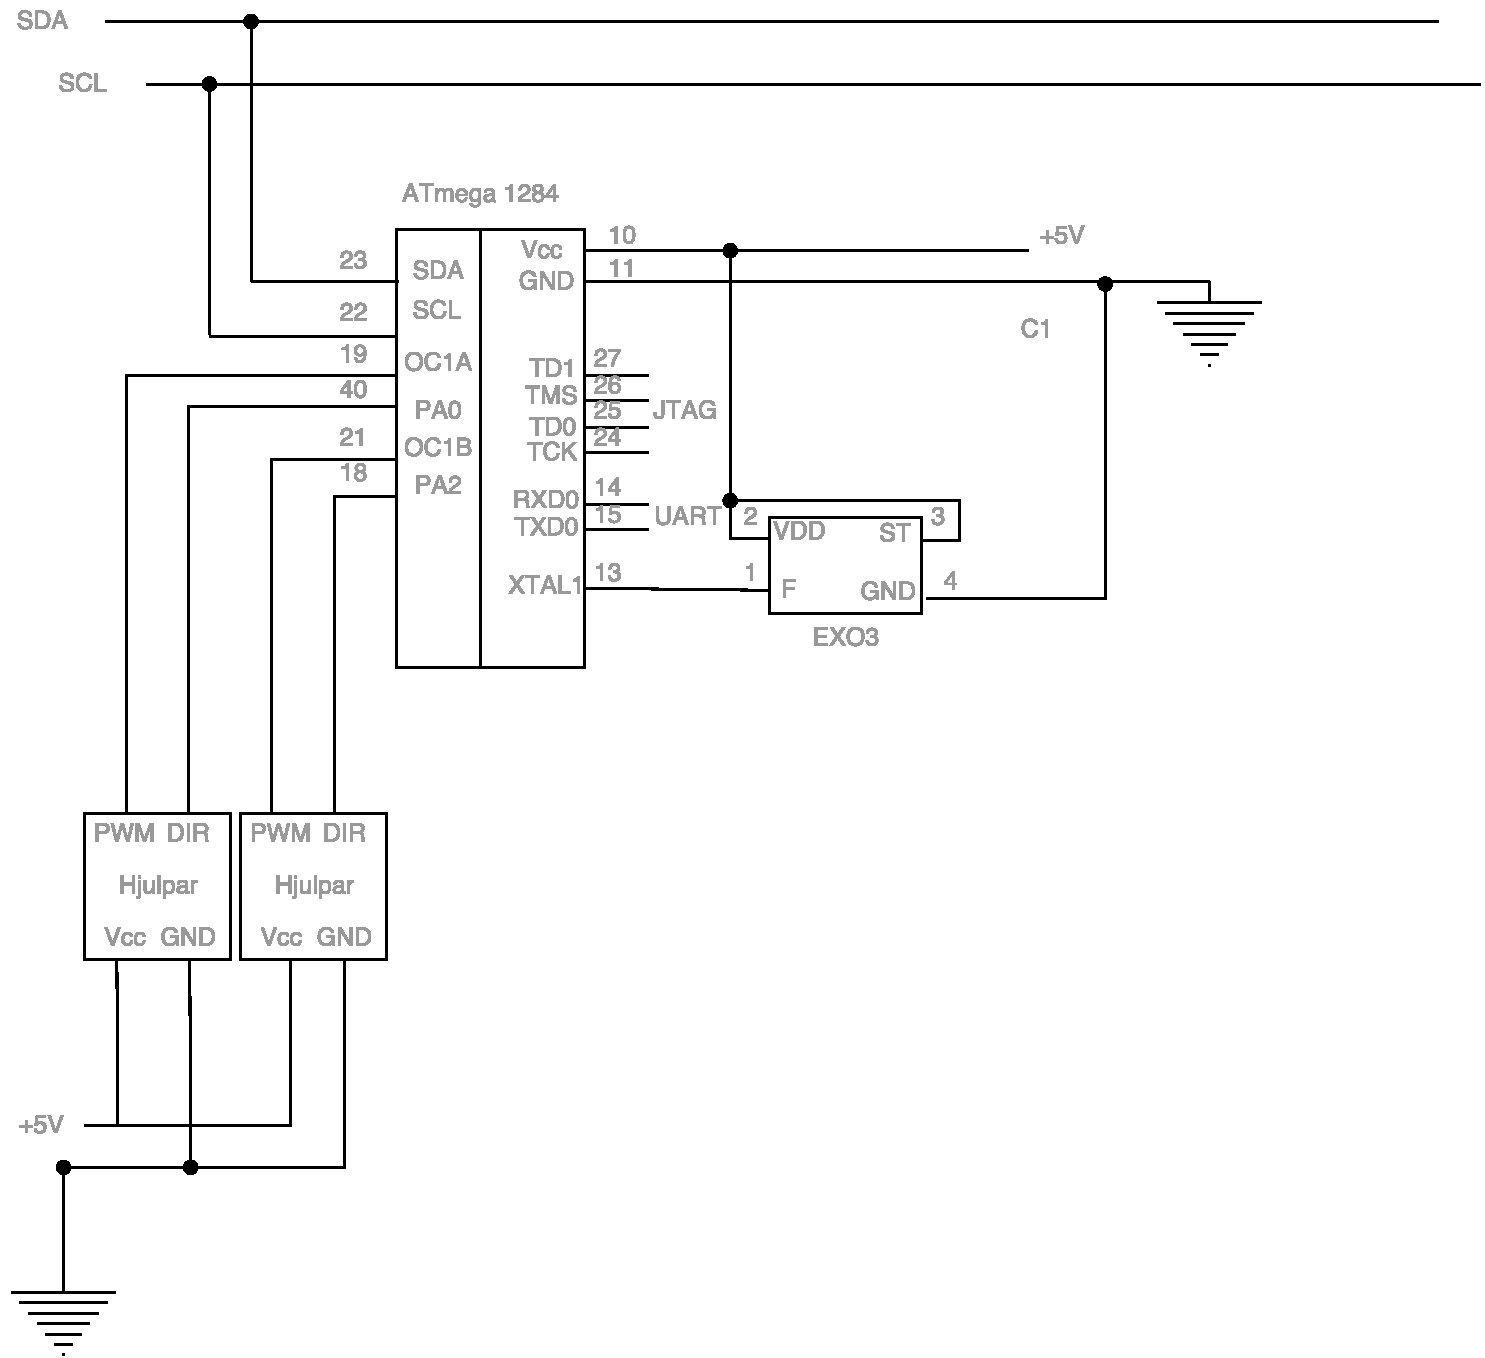
\includegraphics[scale=0.45]{Styrenhet_kopplingsschema}
\caption{Kopplingsschema för styrenheten.}
\label{fig:styrenhet_kopplingsschema}
\end{figure}

TODO:TEXT OM KOPPLINGSSCHEMA

\subsubsection{Komponenter}

\begin{table}[H]
  \centering
  \begin{tabular}{ | c | c |}
    \hline
    \textbf{Komponent} & \textbf{Antal} \\
    \hline
    ATMega 1284 & 1 \\
    \hline
    Terminator (bas för fyrhjulingsrobot) & 1 \\
    \hline
    EXO3 & 1 (delad) \\
    \hline
    LS241 & 1 \\
    \hline
  \end{tabular}
\end{table}


\subsubsection{Resurser}
TODO:TABELL NEDAN EJ KORRIGERAD
\begin{table}[H]
  \centering
  \begin{tabular}{ | c | c | c | c |}
    \hline
    \textbf{Port} & \textbf{Antal} & \textbf{Krävs} \\
    \hline
    SDA & 1 & 1 \\
    \hline
    SCL & 1 & 1 \\
    \hline
    RESET & 1 & 1 \\
    \hline
    IO & 30 & 5 \\
    \hline
    USART & 4 & 4 \\
    \hline
    JTAG & 1 & 1 \\
    \hline
    CLK & 1 & 1 \\
    \hline
  \end{tabular}
  \caption{Tabell över tillgängliga portar på processorn.}
\end{table}

Omvandlingen av kommandon från huvudenheten och utskickning av signaler till servona uppskattas ej kräva mer prestanda eller minne än styrenhetens ATMega 1284 processor klarar av.

\subsubsection{Programflöde}

\begin{figure}[H]
\centering
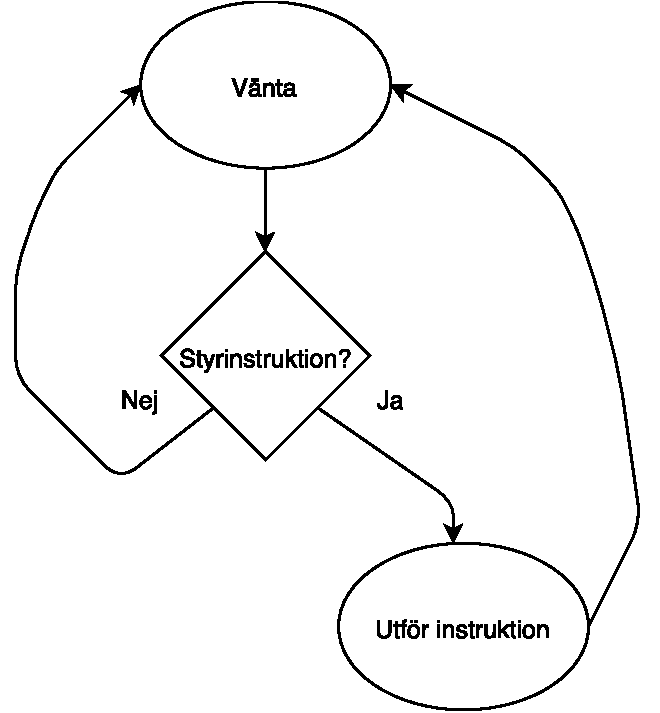
\includegraphics[scale=0.6]{Styrenhet_flowchart}
\caption{Ett flödesschema över styrenhetens tillstånd}
\label{fig:styrenhet_flowchart}
\end{figure}

Styrenheten står hela tiden och väntar på instruktioner från huvudenheten, och så snart den får några utför den dem så snabbt den kan. ett flödesschema över styrenhetens beteende kan ses i figur ~\ref{fig:styrenhet_flowchart}.

\subsection{Presentationsenhet}
% Se kommentarer för huvudenhet
TODO:UPPDATERA TEMPUS

\subsubsection{Delsystemets funktion}
TODO:UPPDATERA TEMPUS


\subsubsection{Blockschema}

% Övergripande schema för systemets stuktur
\begin{figure}[H]

\includegraphics[scale=0.37]{Logo}
\caption{Presentationsenheten i omgivning}
\label{fig:Oversikt_presentationsenhet3}
\end{figure}

TODO:TEXT OM BLOCKSCHEMA SOM REFLEKTERAR IMPLEMENTATION

\subsubsection{Komponenter}
Mjukvaruklienten och därmed presentationsenheten kräver en bärbar dator med Bluetooth. 


\subsubsection{Resurser}
TODO:VI ANVÄNDER INGEN TILLHANDAHÅLLEN BÄRBAR DATOR. KBRY?
Presentationen och behandlingen av datan som presentationsenhet mottager uppskattas ej kräva mer minne eller prestanda än vad den tillhandahållna bärbara datorn klarar av.

\subsubsection{Programflöde}
\begin{figure}[H]
\centering 

\includegraphics[scale=0.3]{Logo}
\caption{Flödesschema över presentationsenheten}
\label{fig:Presentationsenhet3}
\end{figure}

TODO:TEXT OM PROGRAMFLÖDE SOM REFLEKTERAR IMPLEMENTATION

\subsection{Fjärrstyrningsenhet}
% Se kommentarer för huvudenhet
TODO:TEXT SOM SPEGLAR IMPLEMENTATION

\subsubsection{Delsystemets funktion}
TODO:TEXT SOM SPEGLAR IMPLEMENTATION

\subsubsection{Blockschema}
% Övergripande schema för systemets stuktur
\begin{figure}[H]
\centering 

\includegraphics[scale=0.37]{Logo}
\caption{Fjärrstyrningsenheten i omgivning}
\label{fig:Oversikt_fjarrstyrenhet3}
\end{figure}
TODO:TEXT OM BLOCKSCHEMA SOM REFLEKTERAR IMPLEMENTATION

\subsubsection{Komponenter}
Fjärrstyrningsenheten kräver en dator med Bluetooth som kan köra mjukvaruklienten, samt tangentbord och mus/touchpad för interaktion med klienten. 

\subsubsection{Resurser}
TODO:VI ANVÄNDER INGEN TILLHANDAHÅLLEN BÄRBAR DATOR. KBRY?
Funktionaliteten för att ta emot användarinput och skicka iväg den via Bluetooth uppskattas ej kräva mer minne eller prestanda än vad den tillhandahållna datorn klarar av.


\subsubsection{Programflöde}
\begin{figure}[H]
\centering 

\includegraphics[scale=0.3]{Logo}
\caption{Flödesschema över fjärrstyrningssenheten}
\label{fig:Fjarrstyrningsenhet_flowchart3}
\end{figure}

TODO:TEXT OM PROGRAMFLÖDE SOM REFLEKTERAR IMPLEMENTATION

\section{Kommunikation mellan delsystem}
\label{sec:kommunikation_mellan_delsystem}
TODO:UPPDATERA TEMPUS, KANSKE IMPLEMENTATION?

\subsection{Huvudbuss}
TODO: KORREKTURLÄS SÅ DET FORTFARANDE STÄMMER 
Systemets moduler på roboten kommer vara sammankopplade med en I2C-buss (även kallad Two-Wire-Interface) där huvudenheten skickar och tar emot kommandon från sensor- och styrenheten. Huvudbussen kommer även att användas för att skicka sensordata från lasersensorn samt den kombinerade accelerometern och gyrot till sensorenhetens processor.

\subsubsection{Uppbyggnad}
TODO: KORREKTURLÄS SÅ DET FORTFARANDE STÄMMER 
Bussen består så som dess alternativa namn antyder av ett två-trådat gränssnitt och stödjer upp till 128 enheter. De två trådarna är SDA och SCL, där SDA överför data medan SCL styr med vilken frekvens detta sker. SDA kommer skrivas till utav bussens alla inkopplade enheter och behöver kopplas in till ett pull-up-motstånd för att inte flyta. Uppbyggnaden av bussen och dess master-slave förhållande kan ses i figur~\ref{fig:huvudbuss_masterslave}.

\subsubsection{Master-slave roller}
\begin{figure}[H]
\centering 

\includegraphics[scale=0.56]{Logo}
\caption{Huvudbussens uppbyggnad och master-slave förhållande}
\label{fig:huvudbuss_masterslave}
\end{figure}

TODO:UPPDATERA TEMPUS

\subsection{Bluetooth}
\label{sec:bluetooth}
TODO:UPPDATERA TEMPUS

\subsubsection{Handskakning}
\label{sec:handskakning}
\begin{figure}[H]
\centering 

\includegraphics[scale=0.8]{Logo}
\caption{Bluetooth mellan huvudenheten och mjukvaruklienten}
\label{fig:Kommunikation_Bluetooth}
\end{figure}

TODO:TEXT OM HANDSKAKNING SOM REFLEKTERAR IMPLEMENTATION

\subsubsection{Master-slave roller}
\label{sec:bluetooth_master_slave}
TODO:UPDATERA TEMPUS, KANSKE IMPLEMENTATION?

\subsection{Informationsflöde}
TODO:UPPDATERA TEMPUS

\subsubsection{Kommunikation med sensorenhet}
TODO:UPPDATERA TEMPUS

\subsubsection{Kommunikation med mjukvaruklient}
TODO:UPPDATERA TEMPUS

TODO:SE TILL ATT NEDANSTÅENDE LISTA SPEGLAR IMPLEMENTATION
Den data som skickas från mjukvaruklienten är följande
\begin{itemize}
\item Förfrågan om all ny kartdata sedan en viss tidpunkt t
\item Kommandon för att styra roboten
\item Byte av exekveringsläge
\end{itemize}
\ \\

TODO:SE TILL ATT NEDANSTÅENDE LISTA SPEGLAR IMPLEMENTATION
Den data som skickas till mjukvaruklienten är följande
\begin{itemize}
\item All ny kartdata sedan tidpunkt t
\item Kontinuerlig kartdata
\item Kontinuerlig mätdata
\item Kontinuerlig styrdata
\item Verifikation av kommandon
\end{itemize}

TODO:TEXT OM OVANSTÅENDE LISTOR

\nocite{*}
\bibliography{teknisk_dokumentation}{}
\bibliographystyle{plain}

TODO:BYT UT ALLA BILDER FRÅN PLACEHOLDERN LOGO OCH SE ÖVER ATT DE FORTFARANDE ÄR AKTUELLA
TODO:LCDn SKA IN NÅGONSTANS

\end{document}
